\section{Introduction}
\label{sec : intro}
In this work we reproduced an AC/DC converter both using a simulation and a theoretical model. The circuit consisted of a transformer which receives 230V of AC current and a frequency of 50Hz, an envelope detector and a voltage regulator. The circuit should produce a 12V DC output voltage. \\
For the \textit{ngspice} simulation, we used one current controlled current source and a voltage controlled voltage source and  to simulate the transformer. This is connected in series to the envelope detector, consisting of a full-wave bridge rectifier and a capacitor. In turn, this is connected in series to a voltage regulator consisting of diodes and a resistor. This circuit can be seen in Figure ~\ref{fig:circngspice}.\\
\begin{figure}[H] \centering
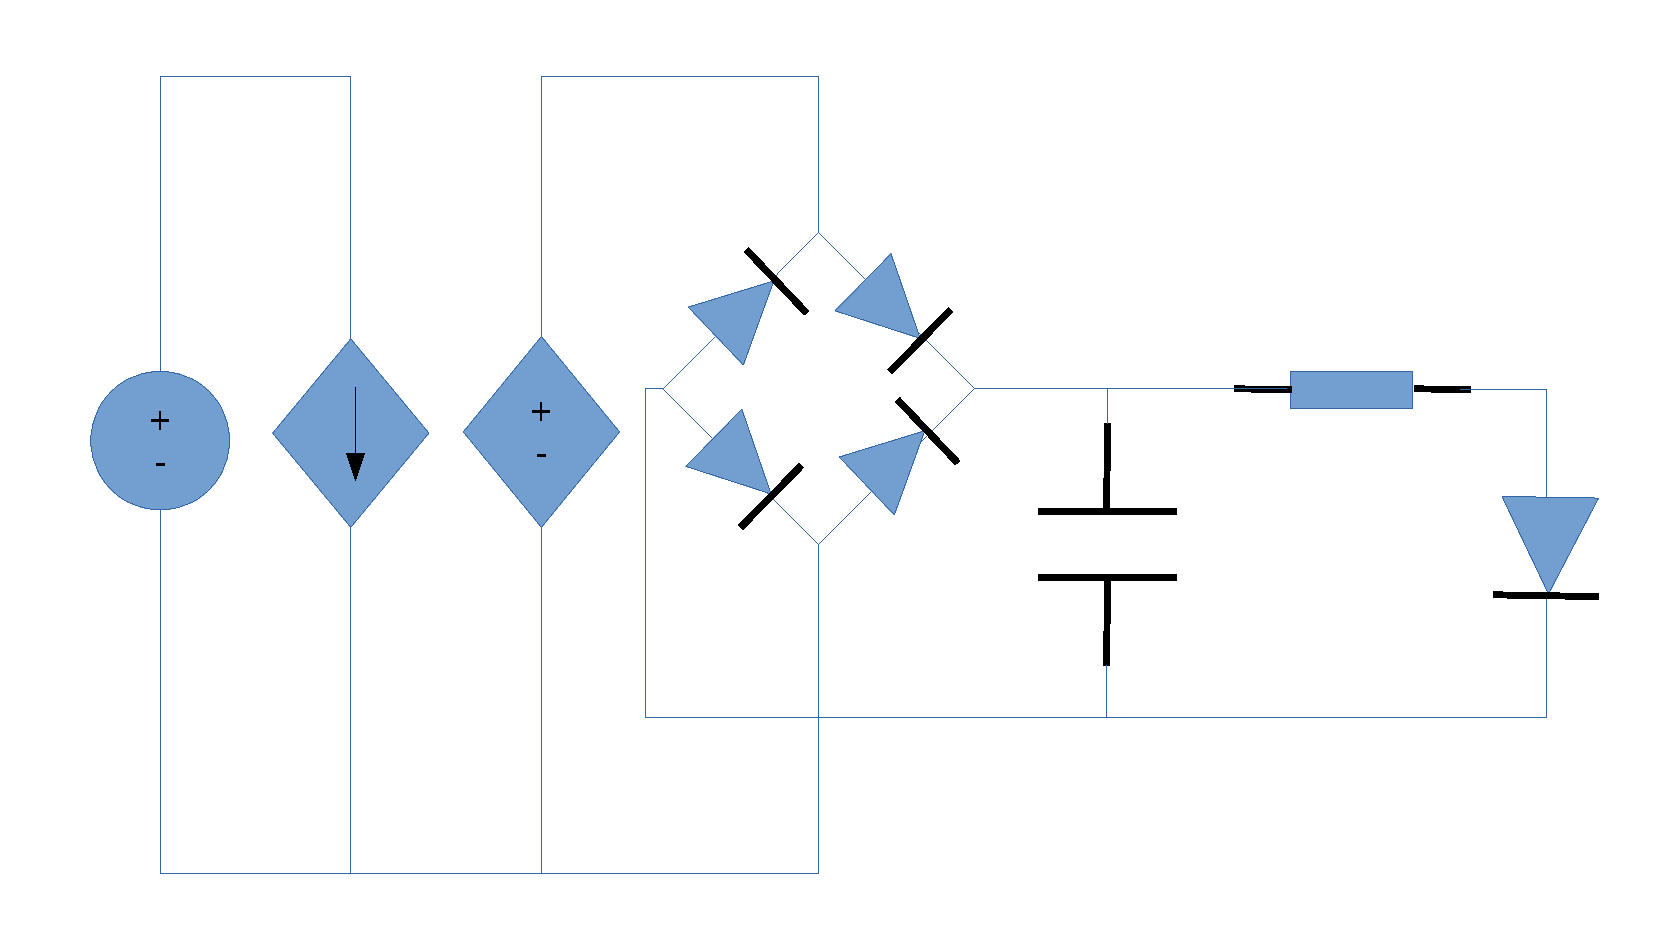
\includegraphics[width=0.8\linewidth]{circngspice.pdf}
\caption{Simulation circuit}
\label{fig:circngspice}
\end{figure} 
In theoretical analysis, the transformer was connected to the same envelope detector, where the diodes were approximated by voltage sources, like the diodes, two in each direction. This circuit can be seen in Figure ~\ref{fig:oc1}, where the voltage source corresponds to the voltage obtained in the secondary winding of the transformer from \textit{ngspice}. In the voltage regulator, seen in Figure ~\ref{fig:oc2}, the same as in the simulation, the diodes were replaced with resistors.\\
\begin{figure}[H] \centering
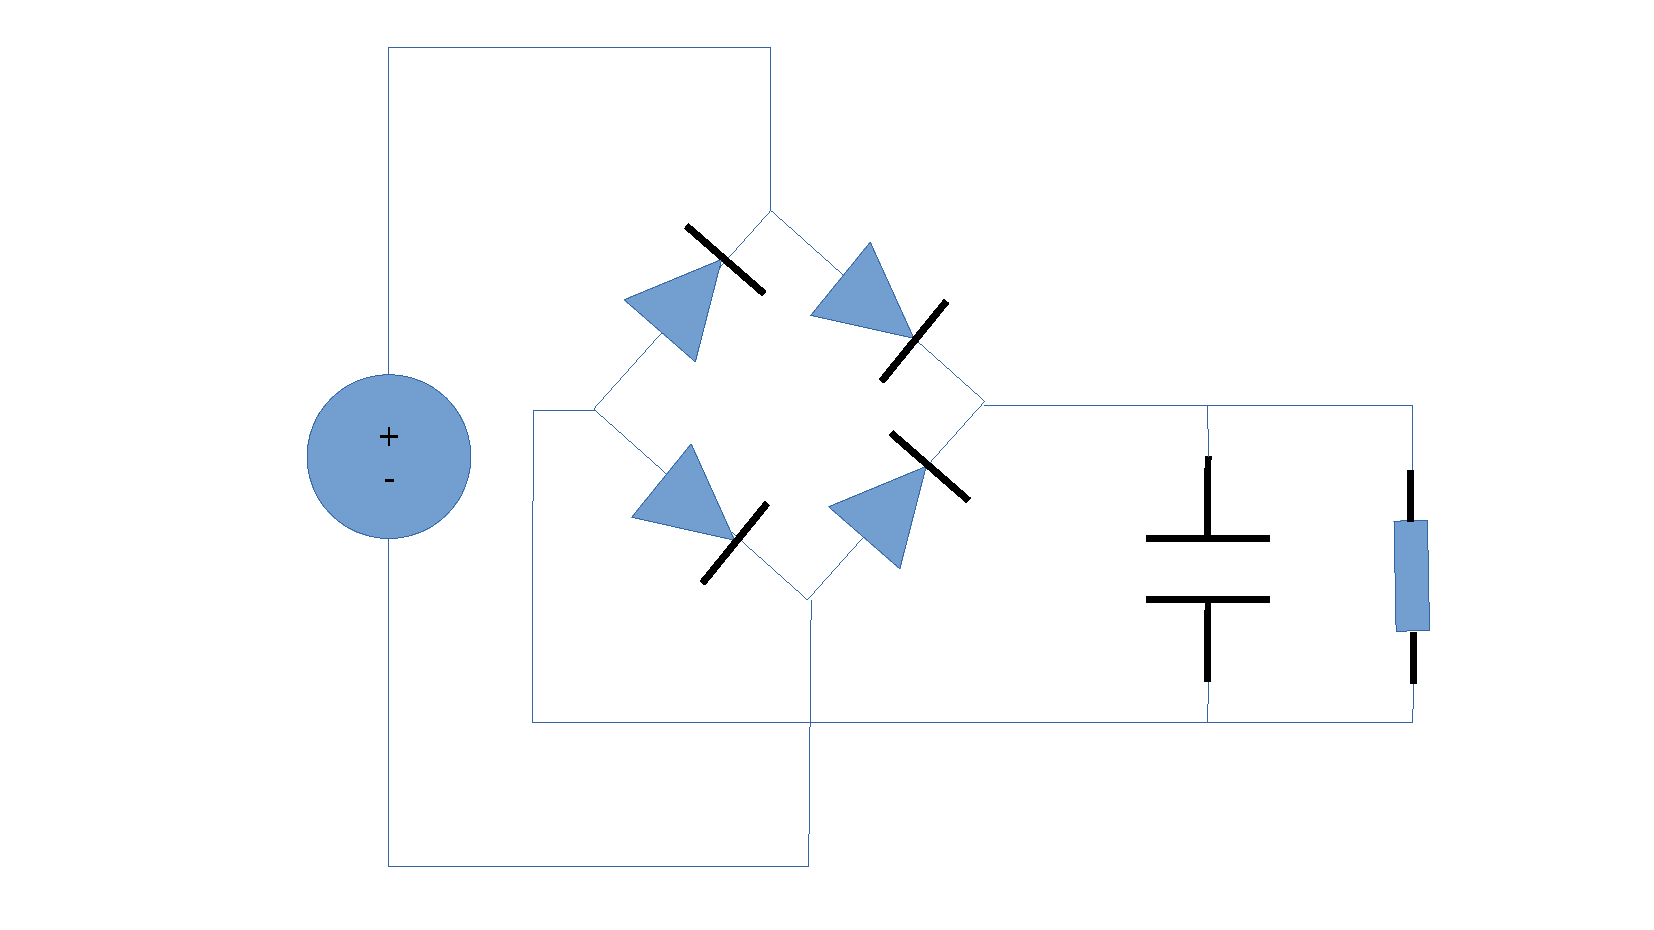
\includegraphics[width=0.8\linewidth]{octave1.pdf}
\caption{Theoretical envelope detector}
\label{fig:oc1}
\end{figure} 

\begin{figure}[H] \centering
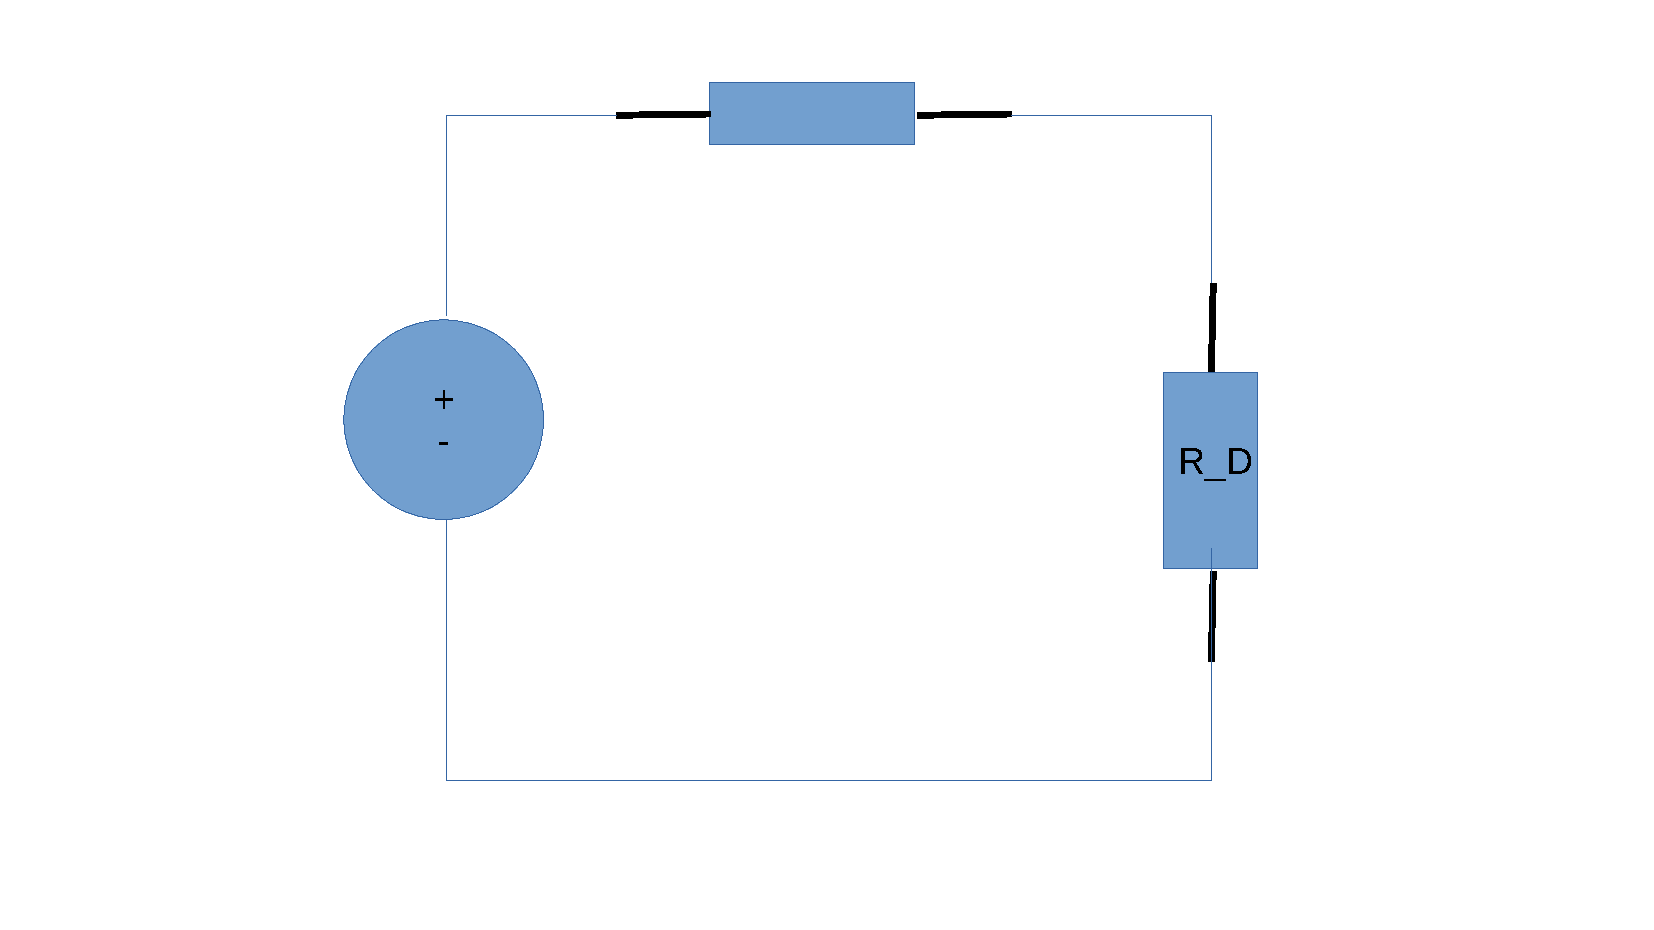
\includegraphics[width=0.8\linewidth]{octave2.pdf}
\caption{Theoretical voltage regulator}
\label{fig:oc2}
\end{figure} 
The comparison between the two methods can be seen in Section ~\ref{sec:res}.
